% Escreva aqui a solução da questão 7.

%\textcolor{red}{ VERSÃO 1 } %Rafaela

Considere o seguinte triângulo de lados $a$, $b$ e $c$, onde $z$, $y$ e $x$ são
suas medianas, respectivamente:

\begin{center}
    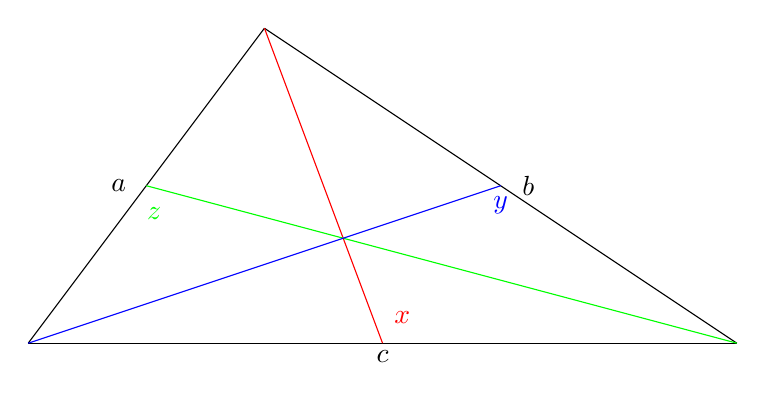
\begin{tikzpicture}
        \draw (0,0) -- (9,0);
        \draw (0,0) -- (3,4);
        \draw (3,4) -- (9,0);
        \node[label=below:{\textbf{$c$}} ] at (4.5,0.15) {};
        \node[label=center:{\textbf{$a$}} ] at (1.15,2) {};
        \node[label=center:{\textbf{$b$}} ] at (6.35,2) {};
        \node[label=below:{\textcolor{red}{\textbf{$x$}}} ] at (4.75,0.65) {};
        \node[label=center:{\textcolor{green}{\textbf{$z$}}} ] at (1.6,1.65) {};
        \node[label=center:{\textcolor{blue}{\textbf{$y$}}} ] at (6,1.75) {};
        \draw[red] (4.5,0) -- (3,4);
        \draw[green] (9,0) -- (1.5,2);
        \draw[blue] (0,0) -- (6,2);
        % \filldraw[red] (1.5,2) circle (0.08);
        % \filldraw[red] (6,2) circle (0.08);
        % \filldraw[red] (4.5,0) circle (0.08);
    \end{tikzpicture}
\end{center}

Queremos provar que: $$x + y + z > \dfrac{a+b+c}{2}.$$ Pela desigualdade
triangular, temos:
\begin{itemize}
    \item  $a < y + \dfrac{b}{2}$ ;
    \item $b < x + \dfrac{c}{2}$;
    \item  $c < z + \dfrac{a}{2}$ .
\end{itemize}
Agora, ``somando'' as desigualdades:
\begin{align*}
    a + b + c < y + x + z + \frac{a}{2} + \frac{b}{2} + \frac{c}{2}
     & \implies a + b + c < y + x + z + \left(\frac{a+b+c}{2}\right) \\
    % & \implies a + b + c - \left(\frac{a+b+c}{2}\right)  < y + x + z + \left(\frac{a+b+c}{2}\right) - \left(\frac{a+b+c}{2}\right)\\
     & \implies \frac{a+b+c}{2} < x+y+z.
\end{align*}
Portanto, provamos que $$x+y+z > \frac{a+b+c}{2}.$$

%\bigskip

%\textcolor{red}{ VERSÃO 2} %autor

%\bigskip

%\textcolor{red}{ VERSÃO 3} % autor

%\bigskip

\bigskip

\textcolor{red}{CHAVE DE PONTUAÇÃO:
    \begin{itemize}
        \item  Uso das 3 desigualdades triangulares \emph{(1,0 ponto)};
        \item Manipulação das inequações \emph{(1,0 ponto)};
        \item  Redação em si (desenho, notação e organização lógica) \emph{(1,0 ponto)}.
    \end{itemize} }